% These packages are optional, depending whether you want the features they provide.
% See the LaTeX Companion or other references for full information.
% !TEX TS-program = pdflatex
% !TEX encoding = UTF-8 Unicode

% This is a simple template for a LaTeX document using the "article" class.
% See "book", "report", "letter" for other types of document.

\documentclass[12pt]{article} % use larger type; default would be 10pt
\usepackage[T2A]{fontenc}
\usepackage[utf8]{inputenc} % set input encoding (not needed with XeLaTeX)
\usepackage[russian]{babel}
%%% Examples of Article customizations
% These packages are optional, depending whether you want the features they provide.
% See the LaTeX Companion or other references for full information.

%%% PAGE DIMENSIONS
\usepackage{geometry}

\usepackage{fancyhdr} 
\geometry{a4paper} % or letterpaper (US) or a5paper or....
% \geometry{margin=2in} % for example, change the margins to 2 inches all round
% \geometry{landscape} % set up the page for landscape
%   read geometry.pdf for detailed page layout information
\usepackage{sectsty}
\usepackage{graphicx} % support the \includegraphics command and options
\usepackage{mathtext}
\usepackage{amsmath}
\usepackage{amsfonts}
% \usepackage[indentfill]{indentskip} % Activate to begin indentagraphs with an empty line rather than an indent
\usepackage{biblatex}
\usepackage{hyperref}
\hypersetup{
  colorlinks=true,
  linkcolor=blue,
  urlcolor=green
}
%%% END Article customizations

%%% The "real" document content comes below...
\usepackage{setspace}
\usepackage[section]{minted}

%%% ToC (table of contents) APPEARANCE
\usepackage[nottoc,notlof,notlot]{tocbibind} % Put the bibliography in the ToC
\usepackage[titles,subfigure]{tocloft} % Alter the style of the Table of Contents

%\date{} % Activate to display a given date or no date (if empty),
         % otherwise the current date is printed 
\usepackage{physics}
\usepackage{float}
\begin{titlepage}
	\thispagestyle{empty}
	\begin{center}
	\large{МИНОБРНАУКИ РОССИИ}\\
	\footnotesize{ФЕДЕРАЛЬНОЕ ГОСУДАРСТВЕННОЕ БЮДЖЕТНОE ОБРАЗОВАТЕЛЬНОЕ УЧРЕЖДЕНИЕ}\\ 
	\footnotesize{ВЫСШЕГО ПРОФЕССИОНАЛЬНОГО ОБРАЗОВАНИЯ}\\ 
	\small{\textbf{«САНКТ-ПЕТЕРБУРГСКИЙ ГОСУДАРСТВЕННЫЙ ПОЛИТЕХНИЧЕСКИЙ УНИВЕРСИТЕТ ПЕТРА ВЕЛИКОГО»}}\\
	\hfill \break
	\normalsize{Институт компьютерных наук и технологий}\\
	\hfill \break
	\normalsize{Высшая школа искусственного интеллекта}\\
	\hfill\break
	\begin{center}
		\normalsize{Дисциплина: \\ПРОГРАММИРОВАНИЕ МИКРОКОНТРОЛЛЕРОВ}
	\end{center}
	\hfill \break
	\hfill \break
	\large{ОТЧЕТ}\\
	\large{По лабораторной работе №2}\\
	\hfill \break
	\hfill \break
	\hfill \break
	\hfill \break
	\hfill \break
	\hfill \break
\end{center}	



\normalsize{ 
	\begin{tabular}{ccc}
		Обучающийся &  гр. 3530201/10001 & Нгуен Куок Дат \\\\
		Руководитель & \hrulefill 				&Вербова Наталья Михайловна\\\\
	\end{tabular}
}\\
\hfill \break
\hfill \break
\hfill \break
\hfill \break
\begin{center} Санкт-Петербург 2022 
\end{center}
\end{titlepage}
\usepackage{indentfirst}
\begin{document}
\begin{center}
\input{titlepage}
\end{center}
\doublespacing
\tableofcontents
\newpage
\section{Цель и постановка задачи}
\subsection{Цель работы}
Ознакомится с основными приемами работы с документацией при составлении программ для микроконтроллеров.
\subsection{Постановка задачи}
\begin{enumerate}
\item Создать проект в Keil, затем подключить заголовочный файл stm32f207xx.h.
\item Проверить работоспособность кода программы, затем снять сигнал с выхода PH6 на осциллогаф.
\item Провести расчет показателей основывая на сигнал с осциллографа
\item Расчеты отразить в отчете
\end{enumerate}

\newpage
\section{Выполнение задания}
\subsection{Код программы}
\inputminted[firstline=1, lastline=18,breaklines ]{C}{F:/git/micro/Lab2/BlinkyLed.c}
\subsection{Измерение волны}
\begin{figure}[H] 
\centering 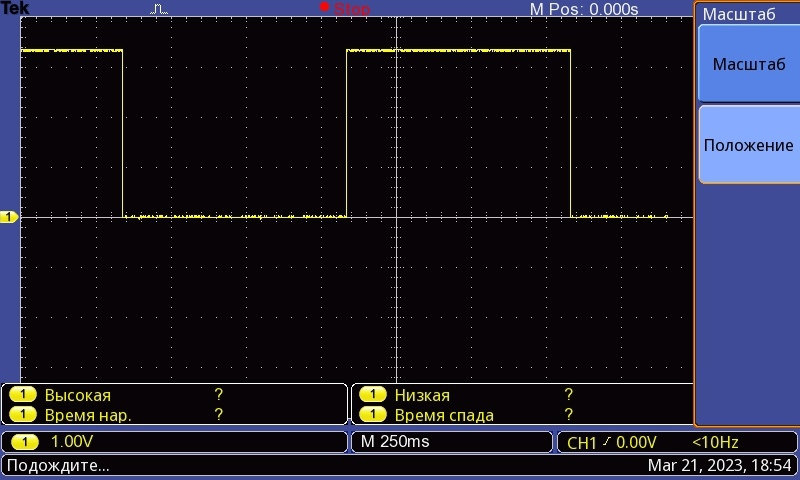
\includegraphics[width = 0.7\textwidth]{graph.jpg}
\end{figure}

 
\[
\begin{align}
& U_\text{ниж} = 3.3V \\
& U_\text{выс} = \~ 0V\\
& \text{Размах} = 3.3V\\
& T_\text{вкл} = 0,250 * 3 = 0,75\text{с} \\
& T_\text{выкл} = 0,250*3 = 0,75\text{с}\\
& К_\text{зап} = 0,5\\
\end{align}
\]



\begin{figure}[H]
\centering 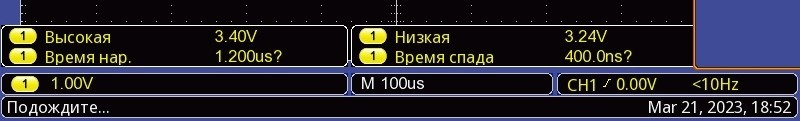
\includegraphics[width = 0.7\textwidth]{slope.jpg}
\end{figure}

\begin{figure}[H]
\centering 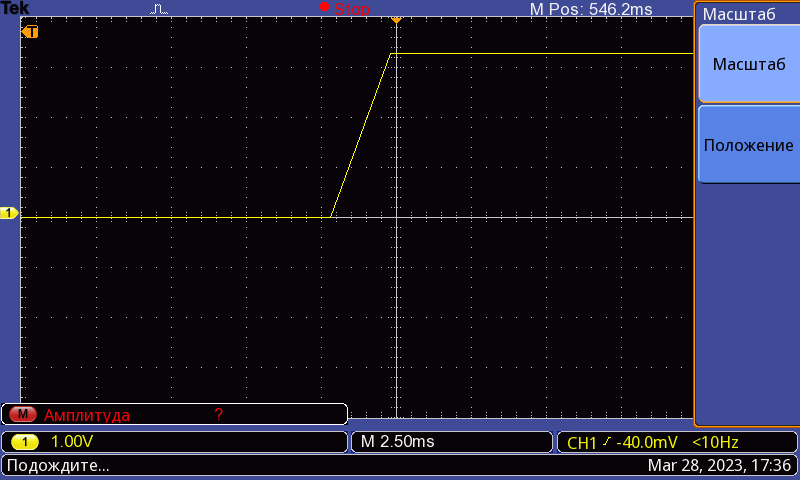
\includegraphics[width = 0.7\textwidth]{slope1.png}
\end{figure}

\begin{figure}[H]
\centering 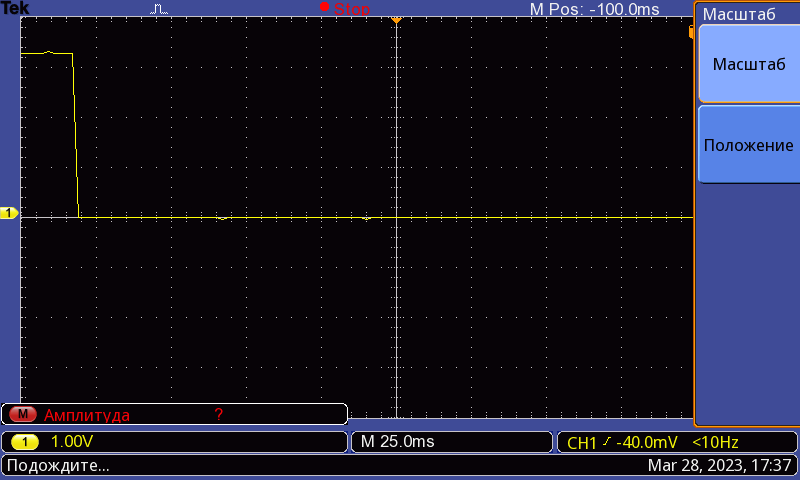
\includegraphics[width = 0.7\textwidth]{slope2.png}
\end{figure}
\[
\begin{align}
& T_\text{нар} = 25\text{mс}\\
& T_\text{спада} = 25\text{mс}\\
\end{align}
\]

\section{Вывод}
В данной работе мы измерили периоды и качественные харктеристики ШИМ сигнала. Коэффициент западывания равно $0,5$,но времени нарастания и спада не равны. 

\end{document}